% figures/ablation-gate.tex — Pareto plot.
% Generated from data/aggregated/{ablation-gate,quality-comparison,baseline-comparison}.csv.
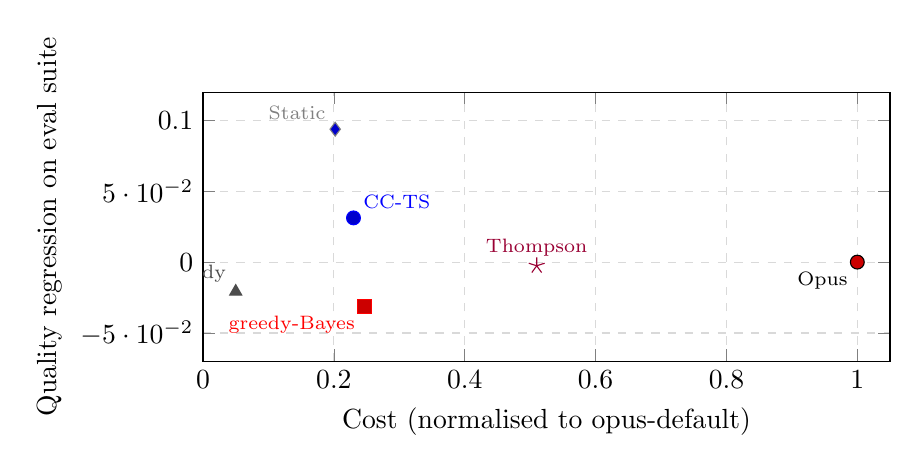
\begin{tikzpicture}
\begin{axis}[
    width=0.85\linewidth, height=5cm,
    xlabel={Cost (normalised to opus-default)},
    ylabel={Quality regression on eval suite},
    xmin=0.0, xmax=1.05,
    ymin=-0.07, ymax=0.12,
    grid=major, grid style={dashed, gray!30},
    legend pos=north west, legend style={font=\scriptsize},
]
\addplot+[only marks, mark=*, mark size=2.5pt, blue]
    coordinates {(0.230, 0.0312)} node[anchor=south west, font=\scriptsize] {CC-TS};
\addplot+[only marks, mark=square*, mark size=2.5pt, red]
    coordinates {(0.247, -0.0312)} node[anchor=north east, font=\scriptsize] {greedy-Bayes};
\addplot+[only marks, mark=star, mark size=3pt, purple!80!black]
    coordinates {(0.510, -0.0026)} node[anchor=south, font=\scriptsize] {Thompson};
\addplot+[only marks, mark=triangle*, mark size=2.5pt, black!70]
    coordinates {(0.050, -0.0208)} node[anchor=south east, font=\scriptsize] {$\varepsilon$-greedy};
\addplot+[only marks, mark=diamond*, mark size=2.5pt, gray]
    coordinates {(0.202, 0.0938)} node[anchor=south east, font=\scriptsize] {Static};
\addplot+[only marks, mark=*, mark size=2.5pt, black]
    coordinates {(1.000, 0.000)} node[anchor=north east, font=\scriptsize] {Opus};
\end{axis}
\end{tikzpicture}
